\documentclass{beamer}
\usetheme{Boadilla} % Clean structure
\useinnertheme{circles} % Dots for sections
\useoutertheme{miniframes} % Header nav with section progress
\setbeamertemplate{navigation symbols}{} % Remove nav icons

\usepackage[utf8]{inputenc}
\usepackage{amsmath, amsfonts, graphicx, booktabs, hyperref}
\usepackage{tikz, caption}
\usepackage{booktabs}
% Custom colors
\definecolor{DeepBlue}{RGB}{0,51,102}
\setbeamercolor{title}{fg=DeepBlue}
\setbeamercolor{frametitle}{fg=DeepBlue}
\setbeamercolor{structure}{fg=DeepBlue}
\setbeamercolor{item}{fg=DeepBlue}

% Frame title underline
\setbeamertemplate{frametitle}{
    \insertframetitle\\
    \vspace{-0.3cm}
    \color{DeepBlue}\rule{\linewidth}{0.2mm}
    \vspace{0.3cm}
}

% Footer with long title and date
\setbeamertemplate{footline}
{
  \leavevmode%
  \hbox{%
  \begin{beamercolorbox}[wd=.20\paperwidth,ht=2.25ex,dp=1ex,center]{author in head/foot}%
    {\fontsize{6}{6} \selectfont Anushka Mukherjee}
  \end{beamercolorbox}%
  \begin{beamercolorbox}[wd=.60\paperwidth,ht=2.25ex,dp=1ex,center]{title in head/foot}%
    \usebeamerfont{title in head/foot}{\fontsize{6}{6}\selectfont Modeling Household Carbon Footprints - August 19, 2025}
  \end{beamercolorbox}%
  \begin{beamercolorbox}[wd=.20\paperwidth,ht=2.25ex,dp=1ex,right]{date in head/foot}%
    {\fontsize{6}{6} \selectfont \insertframenumber{} / \inserttotalframenumber}\hspace*{1em}
  \end{beamercolorbox}}%
  \vskip0pt%
}

% Title info
\title[Modeling Household Carbon Footprints]{Modeling Household Carbon Footprints: Methods, Metrics, and Estimation Frameworks}
\author[Anushka Mukherjee]{Anushka Mukherjee\\Matriculation No: 50075072}
\institute[University of Bonn]{University of Bonn}
\date[July 2025]{Master's Thesis Presentation\\August 19, 2025}

\begin{document}

% Title slide
\begin{frame}
  \titlepage
\end{frame}

% Table of contents
\begin{frame}{Overview}
  \tableofcontents
\end{frame}

% -------------------
\section{Introduction}
\begin{frame}{Motivation}
\vspace{-1.5em}
\small
Households are increasingly recognized as key actors in climate mitigation. However, the methods used to estimate their carbon footprints differ widely.

\begin{columns}
  \begin{column}{0.65\textwidth}
    \begin{itemize}
      \item Existing tools:
      \begin{itemize}
        \item Apply divergent system boundaries  (e.g., direct vs. full life-cycle emissions)
        \item Often double-count emissions 
        \item Fail to account for market feedback or investment-related emissions
      \end{itemize}
    \end{itemize}
  \end{column}
  \begin{column}{0.2\textwidth}
    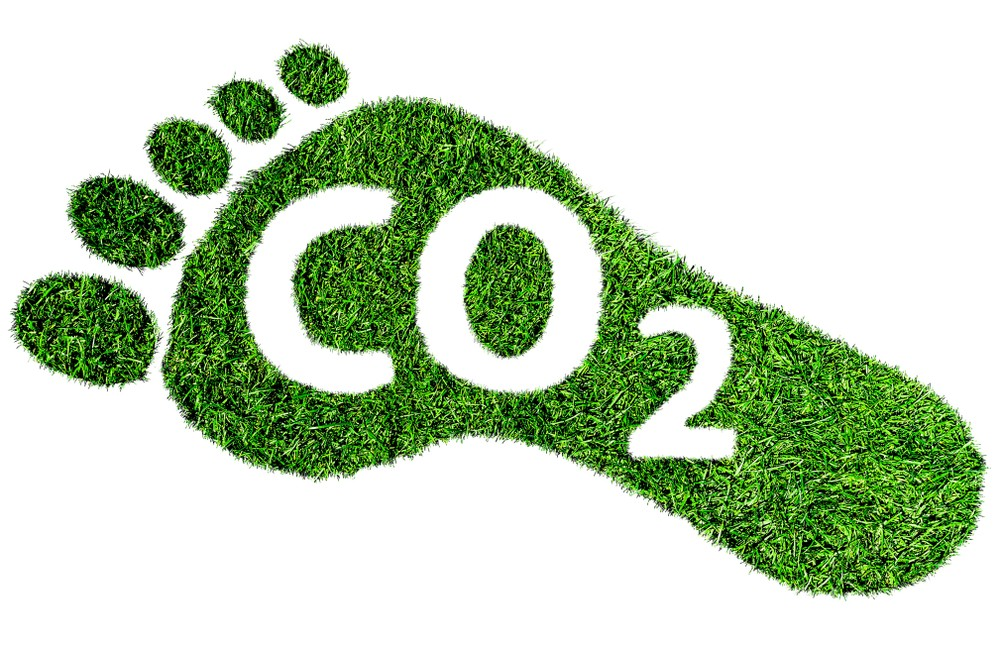
\includegraphics[width=\linewidth]{co2.jpg}
  \end{column}
\end{columns}

\vspace{1em}
\begin{itemize}
\item \small \textbf{Analytical Problem}: The attribution logic embedded in each method fundamentally shapes how household responsibility is quantified.\\
\item \small \textbf{Research Gap}: No unified framework currently compares GHG Protocol, LCA, EEIO, and general equilibrium models from a responsibility perspective.\\
\item \small \textbf{Contribution}: This thesis systematically compares four models to assess attribution differences, empirical consequences, and policy alignment.
\end{itemize}
\end{frame}



% -------------------
\section{Research Questions \& Methodology}
\begin{frame}{Research Questions}
\begin{enumerate}
  \item How do footprint estimates vary across models?
  \item How is household responsibility estimated and attributed under each carbon accounting method?
  \item How do attribution methods shape policy and equity outcomes?
\end{enumerate}
\end{frame}

\begin{frame}{Methodology (I): Analytical Framework}
\small
\vspace{-2.0em}
\begin{itemize}
  \item A comparative framework is used to analyze how different carbon accounting methods attribute household emissions.
  \item The analysis covers four dominant models:
  \begin{itemize}
    \item \textbf{GHG Protocol (Production-based):} Focuses on direct household emissions (Scopes 1–2)
    \item \textbf{Life Cycle Assessment (Product-based):} Attributes emissions across a product's lifecycle
    \item \textbf{EEIO Model (Consumption-based):} Traces emissions through upstream production based on household expenditure
    \item \textbf{Hakenes–Schliephake Model (Consequentialist):} Assigns responsibility based on marginal impact in general equilibrium framework
  \end{itemize}
  \item For each method, the attribution logic, model assumptions, and policy outcomes are compared.
\end{itemize}
\end{frame}

\begin{frame}{Methodology (II): Addressing the Research Questions}
\vspace{-2.5em}
    \small
\textbf{Research Questions Addressed}
\small
\begin{enumerate}[$\Rightarrow$]
  \item \textbf{RQ1:} How do footprint estimates vary across methods?
  \begin{itemize}
    \item Empirical illustrations are derived using official household expenditure data (Eurostat, USDA) and publicly available emission factors (EXIOBASE, Climatiq, IPCC).
    %\item Each method is applied to a harmonized dataset for France, Spain, Germany, and the U.S. wheat sector.
  \end{itemize}
  \item \textbf{RQ2:} How does each method attribute household responsibility?
  \begin{itemize}
    \item Theoretical derivations and decomposition techniques illustrate attribution logic and scope.
    \item Attribution is classified as operational, consumption-based, or consequentialist.
  \end{itemize}
  \item \textbf{RQ3:} What are the equity and policy implications?
  \begin{itemize}
    \item Each attribution model is linked to relevant policy instruments and their distributional impacts.
  \end{itemize}
\end{enumerate}
\end{frame}

\section{Literature Review}
\begin{frame}{Literature Review: Evolution of HCF Estimation}
\small
\vspace{-2.5em}
\begin{itemize}
  \item Research on household carbon footprints (HCF) has expanded since the early 2000s, evolving across three broad phases:
  \begin{itemize}
    \footnotesize
    \item \textbf{Early phase:} IO-based estimation of emissions by expenditure category (Pachauri \& Spreng, 2002; Lenzen, 2004)
    \item \textbf{Expansion:} National comparisons and household heterogeneity (Druckman \& Jackson, 2009; Baiocchi \& Minx, 2010)
    \item \textbf{Integration:} Inequality, global supply chains, and lifestyle effects (Ivanova et al., 2015; Moran et al., 2018)
  \end{itemize}

  \item Dominant methods in current literature:
 
  \begin{itemize}
    \item  \footnotesize \textbf{GHG Protocol:} Activity-based, scope-defined inventories (IPCC Guidelines, 2019)
     \item \footnotesize \textbf{LCA:} Process-based alternative, tracing cradle-to-grave emissions (Steubing et al., 2022)
     \item \footnotesize \textbf{EEIO:} Economy-wide linkages via input–output matrices (Baiocchi \& Minx; 2010, Wiedmann, 2009)
     \item \footnotesize \textbf{GE Models:} Endogenizes household decisions and emissions via market-clearing and investment feedback. (Hakenes \& Schliephake, 2024)
  \end{itemize}
\end{itemize}
\end{frame}


\begin{frame}{Literature Review: Publication Trends and Focus Areas}
\small
\vspace{-2.5em}
\begin{itemize}
  \footnotesize
  \item A bibliometric analysis of \textbf{1,311 peer-reviewed articles (2000–2025)} shows a sharp rise post-2015 (Paris Agreement).
  \item Research is concentrated around \textit{input–output analysis, sustainable consumption}, and \textit{life cycle assessment}.
  \end{itemize}
\vspace{-1.0em}
\begin{columns}
  \centering
  \begin{column}{0.5\textwidth}
    \centering
    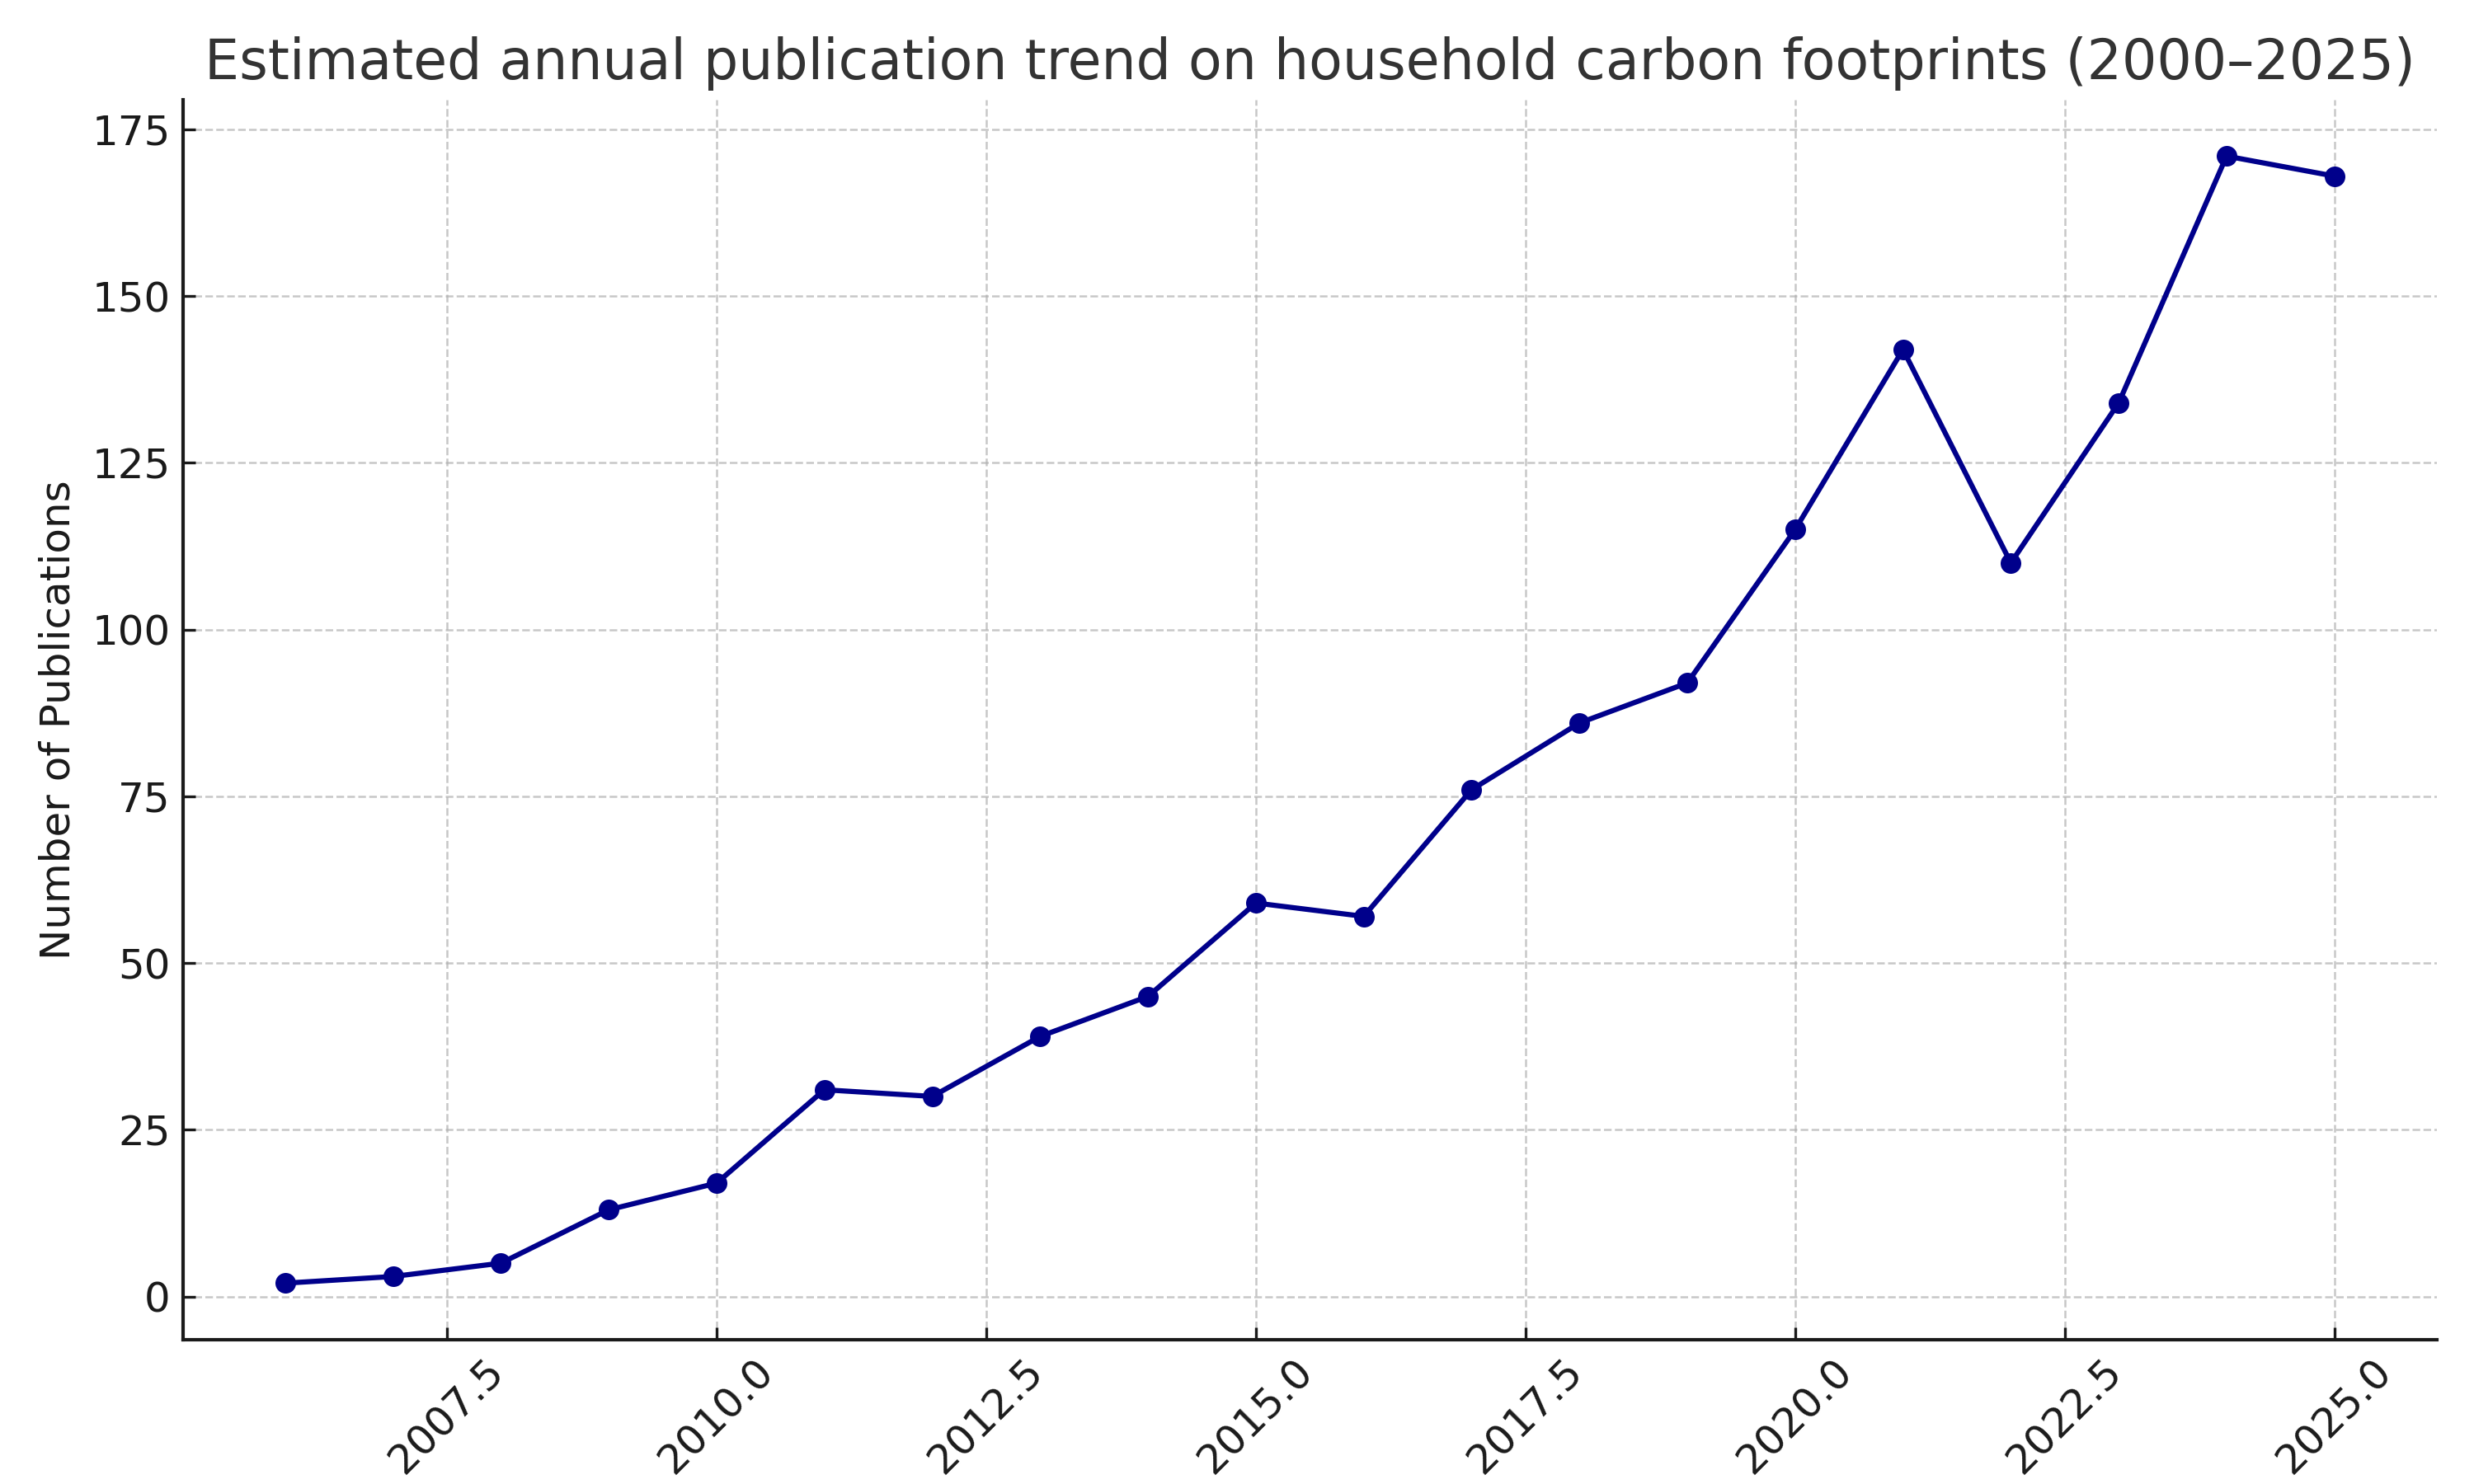
\includegraphics[width=0.8\linewidth]{publication_trend_darkblue_estimated2025.png}
  \end{column}
  \begin{column}{0.6\textwidth}
    \centering
    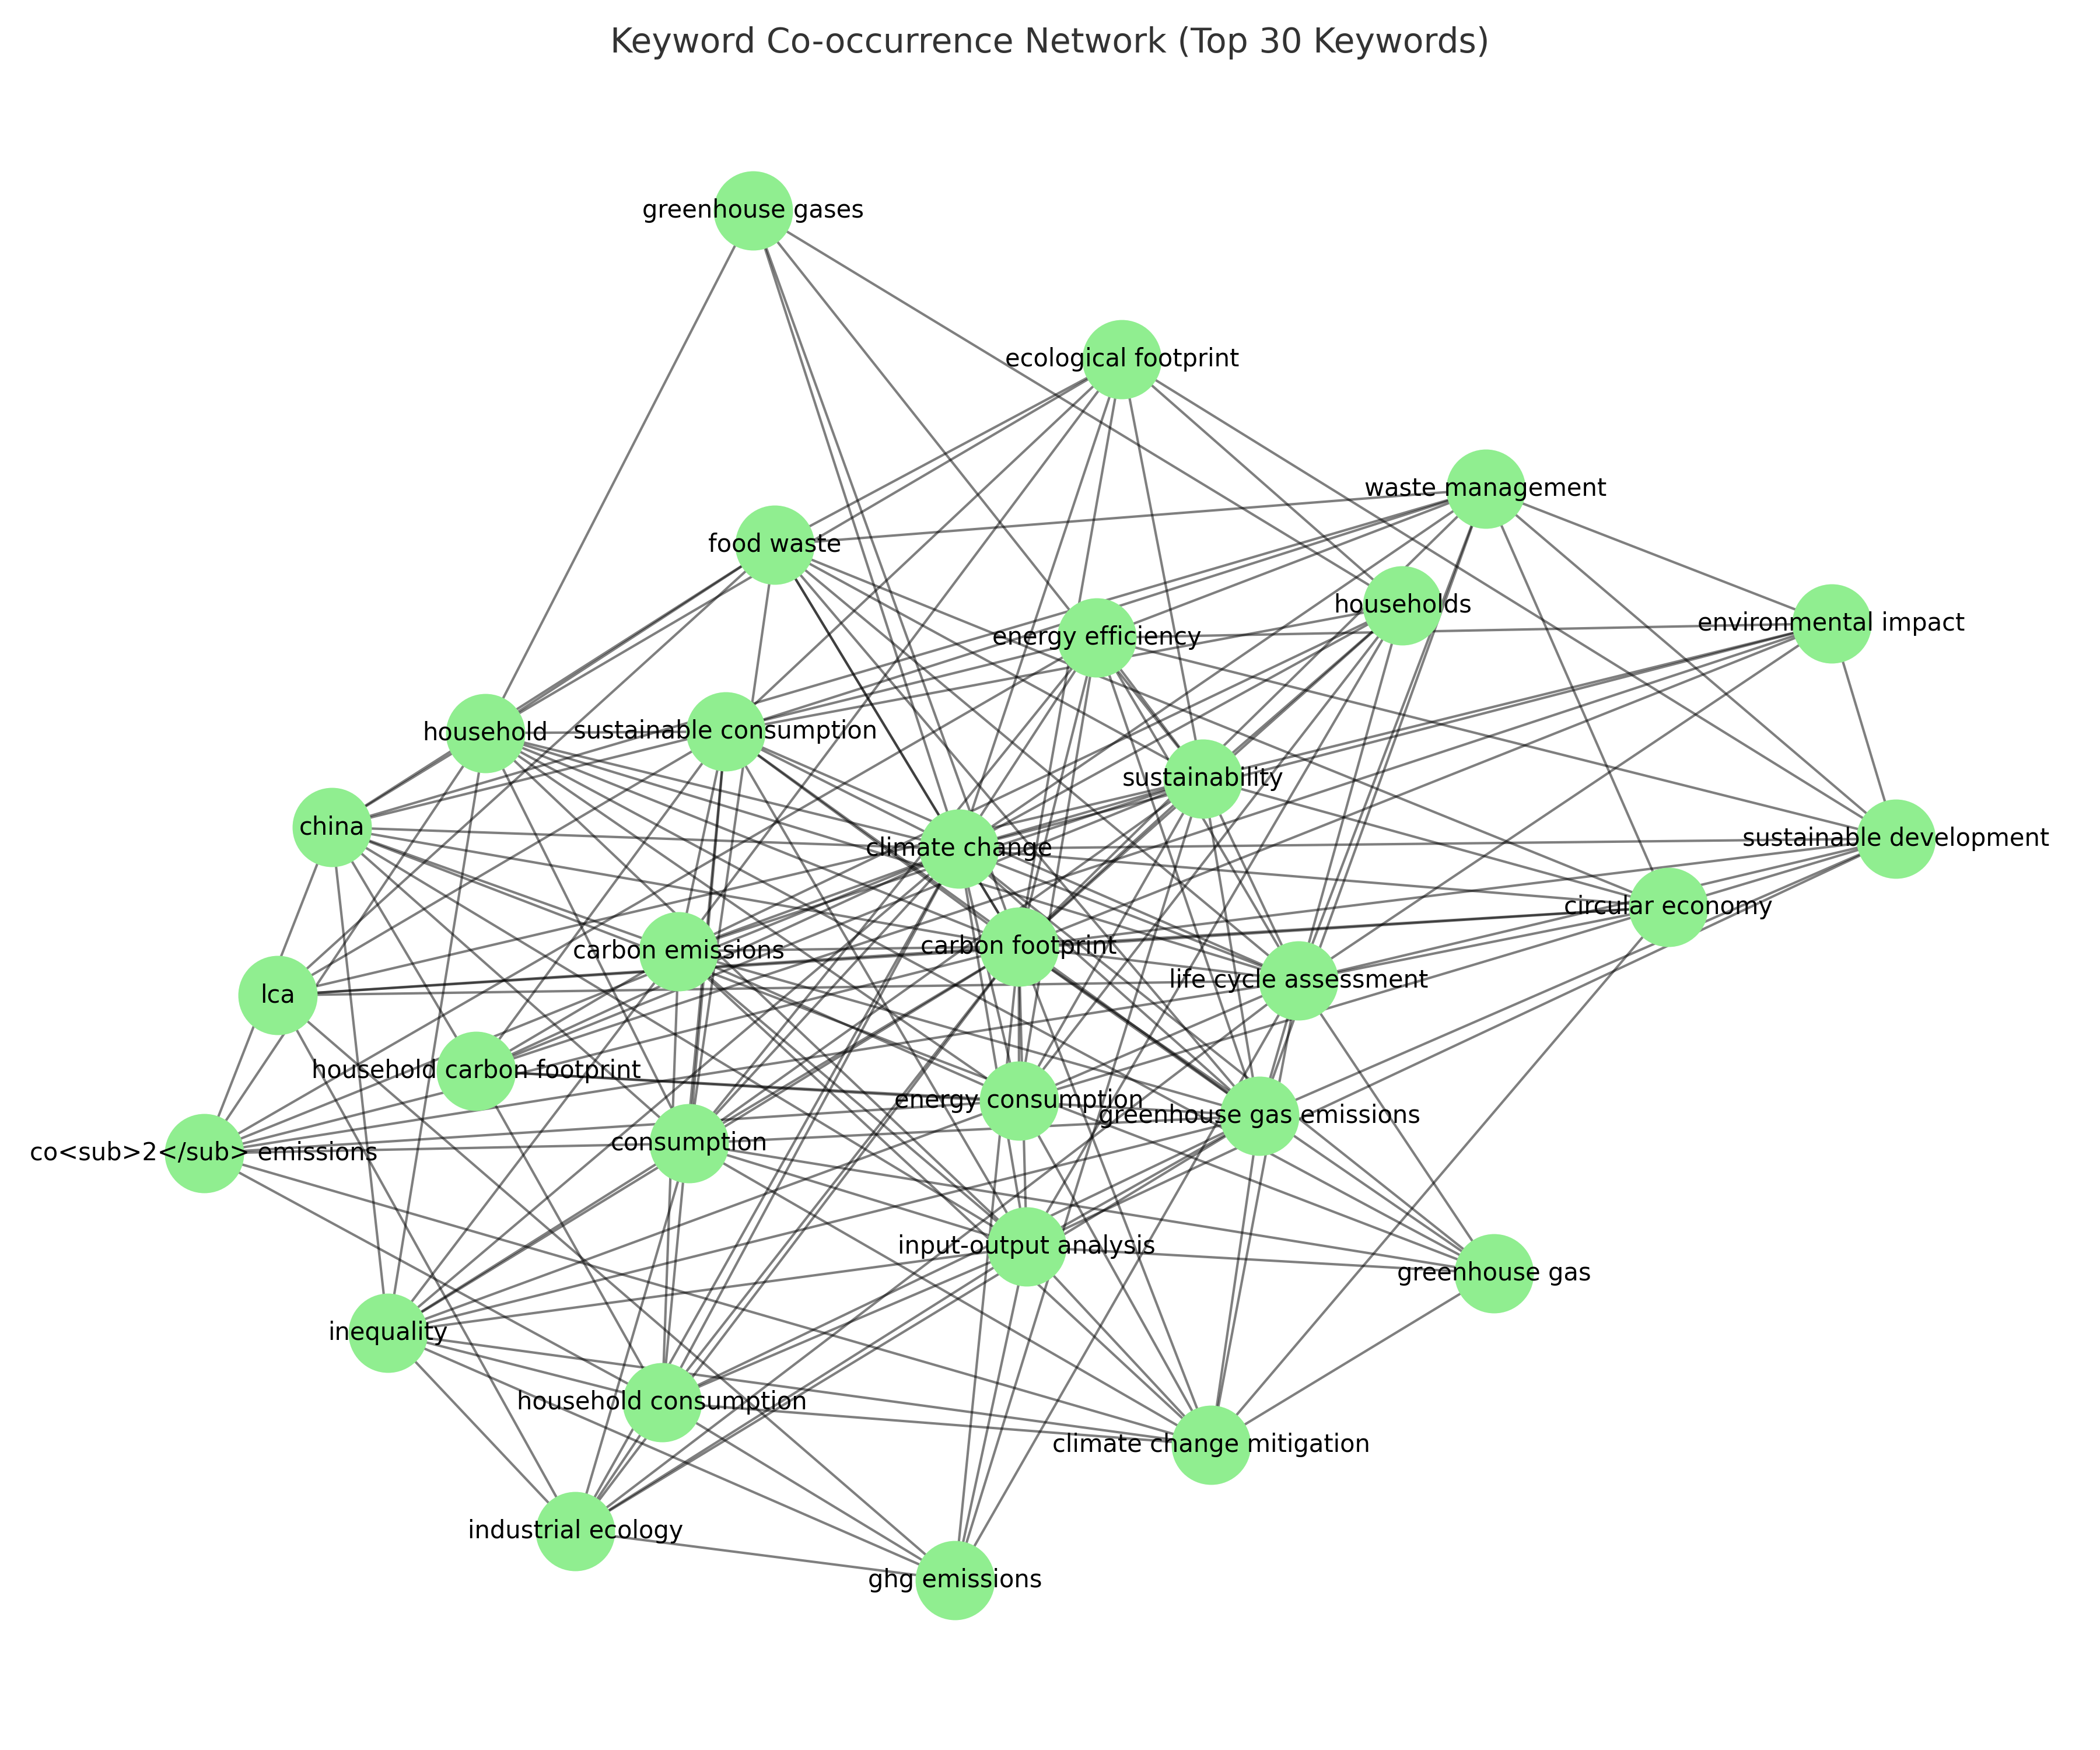
\includegraphics[width=0.7\linewidth]{keyword_cooccurrence.png}
  \end{column}
\end{columns}

\vspace{-0.5em}
\begin{itemize}
  \footnotesize
\item Top Journals: \textit{Journal of Cleaner Production}, \textit{Science of the Total Environment}, and \textit{Environmental Science \& Technology}
  \item Top institutions: University of Tokyo, Sun Yat-sen University, University of Maryland.
\end{itemize}

\end{frame}

\begin{frame}{GHG Protocol: Emission Inventory Framework}
\small
\vspace{-2.5em}

\footnotesize \textbf{Definition:}  
The Greenhouse Gas (GHG) Protocol is a standardized framework developed by WRI and WBCSD for tracking emissions across three scopes.
\vspace{-0.5em}
\begin{figure}[h]
  \centering
  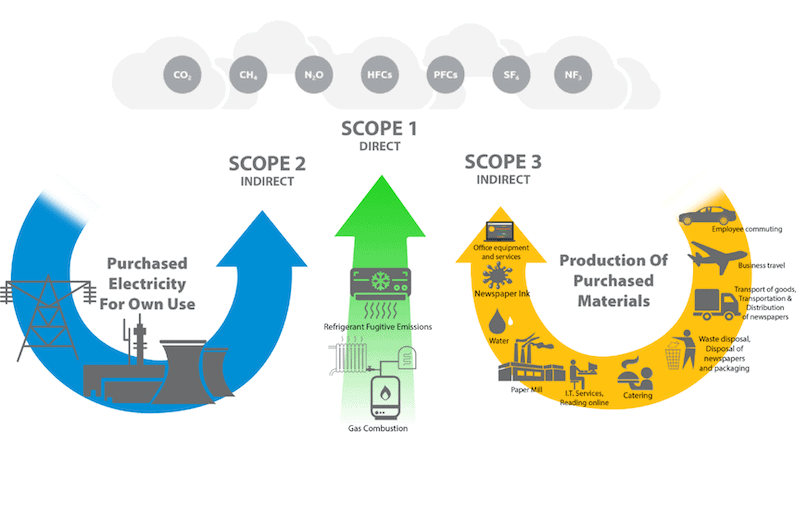
\includegraphics[width=0.55\linewidth]{ghg scope.png}
  \caption*{\tiny Source: Green Element (2023) — https://greenelement.co.uk}
\end{figure}
\vspace{-1.0em}
\footnotesize \textbf{Formulation:}
\[
\text{CF}_{\text{household}} = E_{\text{Scope 1}} + E_{\text{Scope 2}} + E_{\text{Scope 3}}, \quad 
E_i = \sum_j Q_{ij} \cdot EF_{ij}
\]
{\footnotesize where $Q_{ij}$ is the activity level and $EF_{ij}$ is the emission factor for activity $j$ under scope $i$.}

\end{frame}

\section{Methods \& Applications}

\begin{frame}{GHG Protocol – Empirical Application (Spain, 2022)}
\vspace{-2.5em}
  \footnotesize
\textbf{Objective:} Estimate average household emissions by scope using GHG Protocol.

\vspace{0.6em}
\textbf{Data:}  
Spanish household expenditure and energy use (INE 2022), mapped to COICOP categories. Emission factors sourced from DEFRA (2022) and IPCC (2019).

\vspace{0.6em}
\textbf{Method:}
\begin{itemize}
  \item \textbf{Scope 1:} Direct emissions from household fuel combustion (e.g., petrol in vehicles, natural gas for heating).
  \item \textbf{Scope 2:} Indirect emissions from electricity and district heating generation due to household demand.
  \item \textbf{Scope 3:} Indirect emissions from purchased goods and services via € expenditure × emission factor
\end{itemize}

\vspace{0.6em}
\textbf{Avg. annual spending:} = €31,568 \\ 
\textbf{Major spending:} Housing (32.4\%), Food (16\%), Transport (12\%)
\end{frame}

\begin{frame}{GHG Protocol – Empirical Results (Spain, 2022)}
\vspace{-2.0em}
\footnotesize
\textbf{Total Household Carbon Footprint:}  
\[
\text{Total Emissions} = 11,828.08 \text{ kg CO}_2\text{e/year}
\]

\vspace{0.5em}
\textbf{Emissions by Scope}
\begin{table}[h!]
\small
\centering
  \resizebox{\textwidth}{!}{%
\begin{tabular}{lccc}
\toprule
\textbf{Scope} & \textbf{Definition} & \textbf{Emissions (kg CO\textsubscript{2}e)} & \textbf{Share (\%)} \\
\midrule
Scope 1 & Direct fuel use (transport + heating) & 1,114.83 & 9.4\% \\
Scope 2 & Purchased electricity/heating & 829.70 & 7.0\% \\
Scope 3 & Lifecycle emissions from consumption & 9,883.55 & 83.6\% \\
\midrule
\textbf{Total} &  & \textbf{11,828.08} & \textbf{100\%} \\
\bottomrule
\end{tabular}}
\end{table}

\footnotesize
\textbf{Key Findings}
\begin{itemize}
  \item Over 80\% of emissions stem from scope 3 indirect consumption (e.g., food, housing, services).
  \item Scopes 1 and 2 combined account for less than 20\%.
\end{itemize}

\vspace{0.5em}
\textbf{Conclusion:}  
The GHG Protocol effectively captures direct emissions but underestimates total responsibility unless Scope 3 is comprehensively integrated.

%include limitations? Remove the previous slide?
\end{frame}

\begin{frame}{Life Cycle Assessment (LCA): Conceptual Basis}
\footnotesize
\vspace{-0.5em}
\textbf{Definition:}  
Life Cycle Assessment (LCA) calculates greenhouse gas emissions across the full life cycle of a product or service, from resource extraction and production to use and end-of-life disposal.

\vspace{0.7em}
\textbf{Analytical Scope:}  
This method captures both direct and embodied emissions by integrating three complementary approaches:
\begin{itemize}
  \item \textit{Process-based LCA}, which quantifies emissions from discrete production activities such as fuel combustion, agriculture, and food processing
  \item \textit{Input–Output LCA}, which links household consumption to indirect upstream emissions using environmentally extended input–output (EEIO) tables
  \item \textit{Hybrid LCA}, which combines the process-level specificity of traditional LCA with macroeconomic linkages from IO models to reduce system boundary truncation
\end{itemize}

\vspace{0.7em}
\textbf{Carbon Footprint Estimation:}
\[
fp_h = q_h \cdot \text{LCA}_j
\]
where $q_h$ is household consumption and $\text{LCA}_j$ is the unit emission factor for product $j$

\end{frame}

\begin{frame}{Life Cycle Assessment (LCA): Integrated Estimation}
\footnotesize
\vspace{-2.0em}
\textbf{Framework:}  
Adapted from Peng et al. (2021), the hybrid LCA model aggregates activity-based emissions and sequestration:

\[
CF_i = \sum_n E_{in} + \sum_m S_{im}
\quad \text{(emissions + sequestration)}
\]

\vspace{0.3em}
\textbf{Functional Components:}
\begin{itemize}
  \item \textbf{Direct Energy Use:} $E_{id} = \sum_d (F_{id} \cdot EF_d)$
  \item \textbf{Consumption:} Short-lived: $E_{if} = \sum_f (EF_f \cdot C_{if})$  
        Durable: $E_{ij} = \sum_j \frac{EF_j \cdot C_{ij}}{L_j}$
  \item \textbf{Agriculture:} $CF_{ia} = \sum_a EF_a M_{ia} + \sum_t EF_t FS_{ia} + \sum_v B_v \cdot 0.475$
  \item \textbf{Afforestation (Sequestration):} $S_{iaf} = FS_{iaf} \cdot CS_{\text{citrus}}$
  \item \textbf{Livestock:} $E_{il} = \sum_f EF_{if} F_{if} + \sum_l EF_{il} N_{il}$
\end{itemize}

\vspace{0.3em}
\textbf{Implication:}  
The Hybrid LCA structure reduces truncation error and better reflects household-level carbon responsibility particularly in domains such as food, housing, and land use.
\end{frame}

\begin{frame}{LCA Illustration}
\vspace{-2.5em}
\footnotesize
\begin{itemize}
  \item Indirect emissions from food, goods, and services dominate household carbon footprints highlighting the limits of focusing solely on energy behavior.
\end{itemize}
\begin{center}
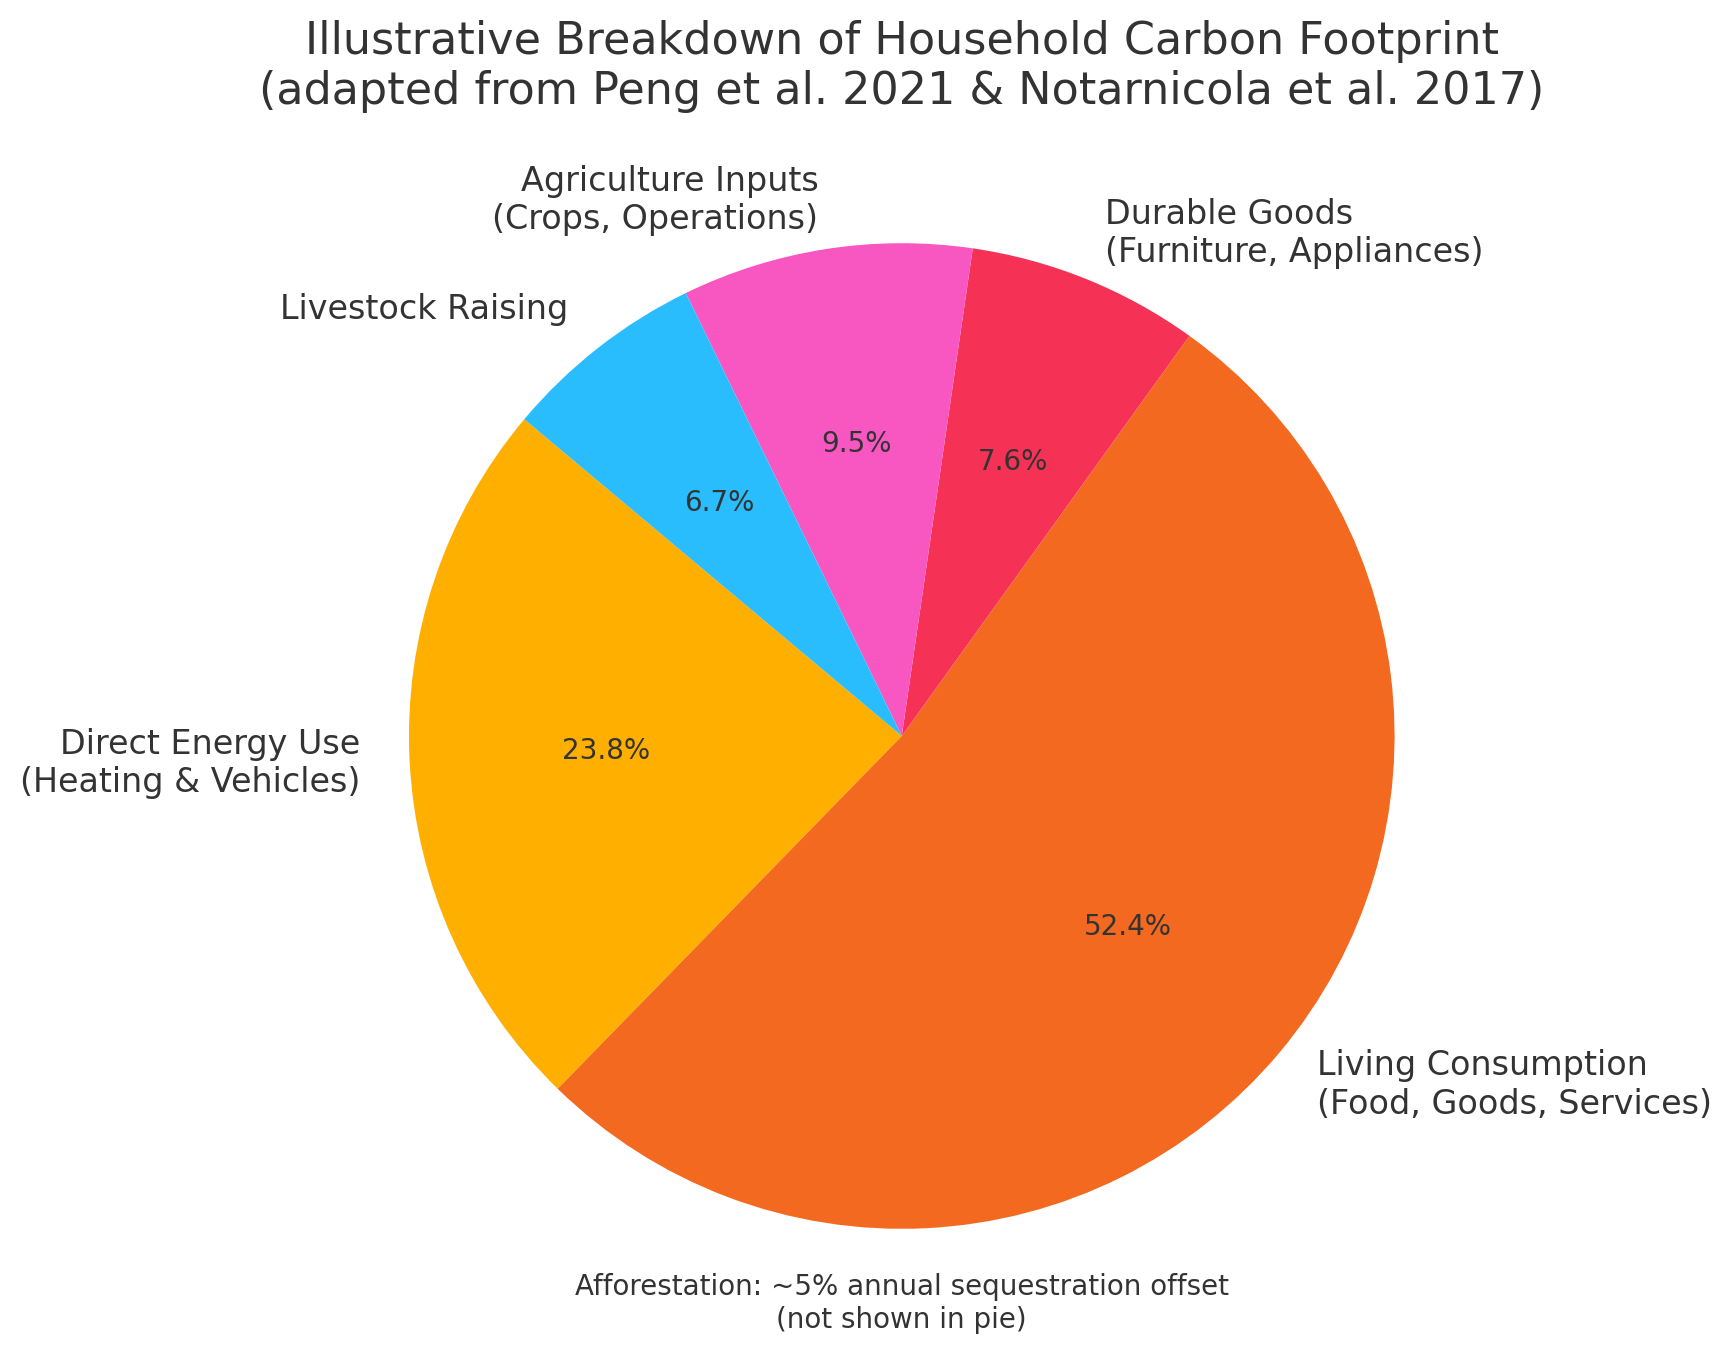
\includegraphics[width=0.68\linewidth]{LCA_pie.png}
\end{center}


\end{frame}

\begin{frame}{Environmentally Extended Input–Output (EEIO) Framework}
\footnotesize
\vspace{-2.5em}
\textbf{Definition:}  
The EEIO model quantifies household carbon footprints by tracing both direct and upstream emissions embedded in goods and services using macroeconomic inter-industry linkages.

\vspace{0.5em}
\textbf{Core Identity:}
\[
\mathbf{X} = (\mathbf{I} - \mathbf{A})^{-1} \cdot \mathbf{F}
\quad
\Rightarrow
\quad
\mathbf{E} = \mathbf{C} \cdot (\mathbf{I} - \mathbf{A})^{-1} \cdot \mathbf{F}
\]

\vspace{0.5em}
\textbf{Components:}
\begin{itemize}
  \item \( \mathbf{A} \): Technical coefficient matrix gives the economic input structure
  \item \( \mathbf{F} \): Final demand vector captures household expenditure
  \item \( \mathbf{C} \): Emission intensity vector (kg CO\textsubscript{2}e / € output)
\end{itemize}

\vspace{0.5em}
\vspace{0.5em}
\textbf{Model Assumptions and Stability:}
\begin{itemize}
  \item Fixed production coefficients (Leontief structure)
  \item No substitution across sectors or inputs
  \item The matrix \( \mathbf{A} \) must satisfy \( \rho(\mathbf{A}) < 1 \) for stability
  \item Empirically: \( \sum_i A_{ij} < 1 \) for all \( j \)
\end{itemize}

\end{frame}

\begin{frame}{EEIO Emissions Decomposition: Tiered Attribution}
\footnotesize
\vspace{-2.0em}
Following Matthews et al. (2008) and Long et al. (2019), household emissions are decomposed into three analytical tiers:

\vspace{0.5em}
\textbf{Tier 1 – Direct Emissions:}
\[
\mathbf{E}_1 = \mathbf{C}_d \cdot \mathbf{F}_d
\quad \text{(e.g., direct fuel use)}
\]

\textbf{Tier 2 – Indirect Energy:}
\[
\mathbf{E}_2 = \mathbf{C}_e \cdot (\mathbf{I} - \mathbf{A})^{-1} \cdot \mathbf{F}_e
\quad \text{(e.g., electricity, heating)}
\]

\textbf{Tier 3 – Indirect Supply Chain:}
\[
\mathbf{E}_3 = \mathbf{C} \cdot \left[(\mathbf{I} - \mathbf{M})(\mathbf{I} - \mathbf{A})\right]^{-1} \cdot \left[(\mathbf{I} - \mathbf{M}) \cdot \mathbf{F} + \mathbf{EX}\right]
\]

\vspace{0.5em}
\textbf{Total Household Footprint:}
\[
\mathbf{E}_{\text{total}} = \mathbf{E}_1 + \mathbf{E}_2 + \mathbf{E}_3
\]

\vspace{0.5em}
\textbf{Note:}  
Import-adjusted tiers ensure that emissions are attributed to domestic demand. Enables national-scale footprint analysis with high coverage.

\end{frame}

\begin{frame}{EEIO Illustration: Method and Aggregate Estimates}
\vspace{-2.0em}
  \footnotesize
\textbf{Methodology:}
\begin{itemize}
  \item Emission intensities \(EF_i\) reflect \( \mathbf{C}(\mathbf{I}-\mathbf{A})^{-1} \), derived from EXIOBASE (via Climatiq.io).
  \item National consumption \(F_{i,c}\) from Eurostat (2021) is multiplied by category-specific \(EF_i\) for each country:
  \[
  E_{i,c} = F_{i,c} \cdot EF_i
  \]
  \end{itemize}

\vspace{0.6em}
\textbf{Total Household Carbon Footprints (2021):}

\begin{table}[h]
\footnotesize
\begin{tabular}{lcc}
\toprule
\textbf{Country} & \textbf{Expenditure (bn €)} & \textbf{Emissions (Mt CO\textsubscript{2}e)} \\
\midrule
France   & 1322.0 & 420.0 \\
Spain    & 747.9  & 227.0 \\
Germany  & 1794.8 & 545.9 \\
\bottomrule
\end{tabular}
\end{table}

\vspace{0.3em}
\footnotesize Source: Eurostat (2021), EXIOBASE (2025); Author’s calculations.
\end{frame}

\begin{frame}{EEIO Illustration: Interpretation of Results}
\small
\vspace{-2.5em}
\textbf{Sectoral Composition of Emissions}
\begin{itemize}
  \item Housing, food, and transport consistently emerge as the most emission-intensive categories.
  \item These three sectors jointly account for over 60\% of total household carbon footprints in France, Spain, and Germany.
\end{itemize}

\vspace{0.6em}
\textbf{Cross-Country Differences}
\begin{itemize}
  \item \textbf{Germany:} Highest absolute emissions, reflecting both higher household expenditure and carbon-intensive energy use.
  \item \textbf{France:} Lower footprint per euro spent, can be attributed to cleaner energy mix and less carbon-intensive consumption.
  \item \textbf{Spain:} Intermediate values, with emissions closely tied to transport and agri-food supply chains.
\end{itemize}



\vspace{0.3em}
\textit{The EEIO framework captures upstream emissions embedded in household consumption, providing a robust basis for cross-country comparison.}
\end{frame}

%------------------------------------------------
\begin{frame}{The Hakenes \& Schliephake Model}
\footnotesize
\vspace{-2.5em}
The model captures the \textit{marginal causal impact} of household behaviour on total emissions, accounting for both \textbf{consumption} and \textbf{investment} channels in a general equilibrium setting.

\vspace{0.4em}
\textbf{Model Assumptions:}
\begin{itemize}
  \item One homogeneous good produced with capital only, constant returns to scale.
  \item Linear technology: \( I = c Q \), where \(Q\) is total output and \(I\) total investment.
  \item Emissions proportional to output: \( X = x Q \).
\end{itemize}

\textbf{Households:}
\begin{itemize}
  \item Wealth \(w\) allocated to consumption \(q_h\) and investment \(i_h\), residual in risk-free asset (\(r_f\)).
  \item Firms raise \(I\) from households, repay with \(r = \frac{P}{c} + \lambda + \varepsilon\), with \(\varepsilon \sim \mathcal{N}(0,\sigma^2)\).
  \item Utility:  
  \[
  U_h = \mathbb{E}\left[-\exp\left(-\alpha \left( a q_h - \frac{b}{2}q_h^2 + m_h - xQ \right)\right)\right]
  \]
\end{itemize}

\textbf{First-Order Conditions:}
\[
q_h = \frac{a - x - P}{b}, \quad 
i_h = \frac{1}{\alpha\sigma^2}\left(\frac{P}{c} + \lambda - r_f\right)
\]
These capture optimal consumption and investment given prices, risk, and emissions.
\end{frame}
%------------------------------------------------

\begin{frame}{Market Equilibrium and Footprint Derivation}
\footnotesize
\vspace{-2.5em}
\textbf{Market Clearing:}
\[
Q = q_h + (n-1)q_{-h}, \quad I = i_h + (n-1)i_{-h}, \quad I = c Q
\]
From other households’ FOCs:
\[
q_{-h} = \frac{a - x - P}{b}, \quad i_{-h} = \frac{1}{\alpha\sigma^2}\left(\frac{P}{c} + \lambda - r_f\right)
\]
Total investment:  
\[
I = \frac{n-1}{\alpha\sigma^2}\left(\frac{P}{c} + \lambda - r_f\right) \quad \Rightarrow \quad Q = \frac{n-1}{c\alpha\sigma^2}\left(\frac{P}{c} + \lambda - r_f\right)
\]

\vspace{0.3em}
\textbf{Supply Curve:}
\[
P = c(r_f - \lambda) + \frac{c^2\alpha\sigma^2}{n-1} Q
\]

\vspace{0.3em}
\textbf{Solving Supply \& Demand:}
\[
Q = (n-1)\frac{a - x - c(r_f - \lambda)}{b + c^2\alpha\sigma^2} + \phi q_h + (1-\phi)\frac{i_h}{c}
\]
where:
\[
\phi = \frac{b}{b + c^2\alpha\sigma^2}
\]

\vspace{0.3em}
\textbf{Consequentialist Footprint:}
\[
fp_h = x\left(\phi q_h + (1-\phi)\frac{i_h}{c}\right), \quad \sum_h fp_h = x Q
\]
\textit{Interpretation:} \(\phi \to 1\) → footprint purely consumption-driven; \(\phi \to 0\) → purely investment-driven. Comparative statics show \(\phi\) ↓ with higher risk aversion (\(\alpha\)) or volatility (\(\sigma^2\)), ↑ with stronger diminishing marginal utility (\(b\)).
\end{frame}
%------------------------------------------------

%---------------------------------------------
\begin{frame}{Empirical Illustration: U.S. Wheat Market}
\footnotesize
\vspace{-2.5em}
\textbf{Objective:} Apply the single-industry Hakenes--Schliephake model to quantify the impact of supply shocks on the carbon footprint.

\vspace{0.5em}
\textbf{Data \& Market Setup:}
\begin{itemize}
  \item USDA (2010--2017): production volumes (supply), total domestic use (demand), average farm-gate wheat prices.
  \item FAO/USDA: emission factor of 10.88~kg~CO\textsubscript{2}e per bushel.
\item Simulated a 15.6\% production shock (2016–2017).
\item \textbf{Carbon Footprint Calculation: }$
\text{Emissions} = Q_{\text{eq}} \times 10.88 \text{ kg CO\textsubscript{2}e/bushel}
$

\end{itemize}


\textbf{Empirical Supply Curve:}
\begin{itemize}
  \item Estimated by OLS: \( P = \beta_0 + \beta_1 Q \).
  \item Demand curve: calibrated linear slope from dataset averages.
  
\end{itemize}

\textbf{Theoretical Supply Curve:}
\[
P(Q) = c(r_f - \lambda) + \frac{c^2 \alpha \sigma^2}{n - 1} Q
\]
\begin{itemize}
  \item Parameters: \(c = 4\), \(r_f = 0.05\), \(\lambda = 0.01\), \(\alpha = 0.5\), \(\sigma = 0.4\), \(n = 100{,}000\).
  \item Demand curve identical to empirical case.
  \item Captures optimal household capital allocation under risk.
\end{itemize}
\end{frame}

%---------------------------------------------

\begin{frame}{Methodology: Empirical vs. Theoretical Supply}
\footnotesize
\vspace{-3.0em}
\begin{center}
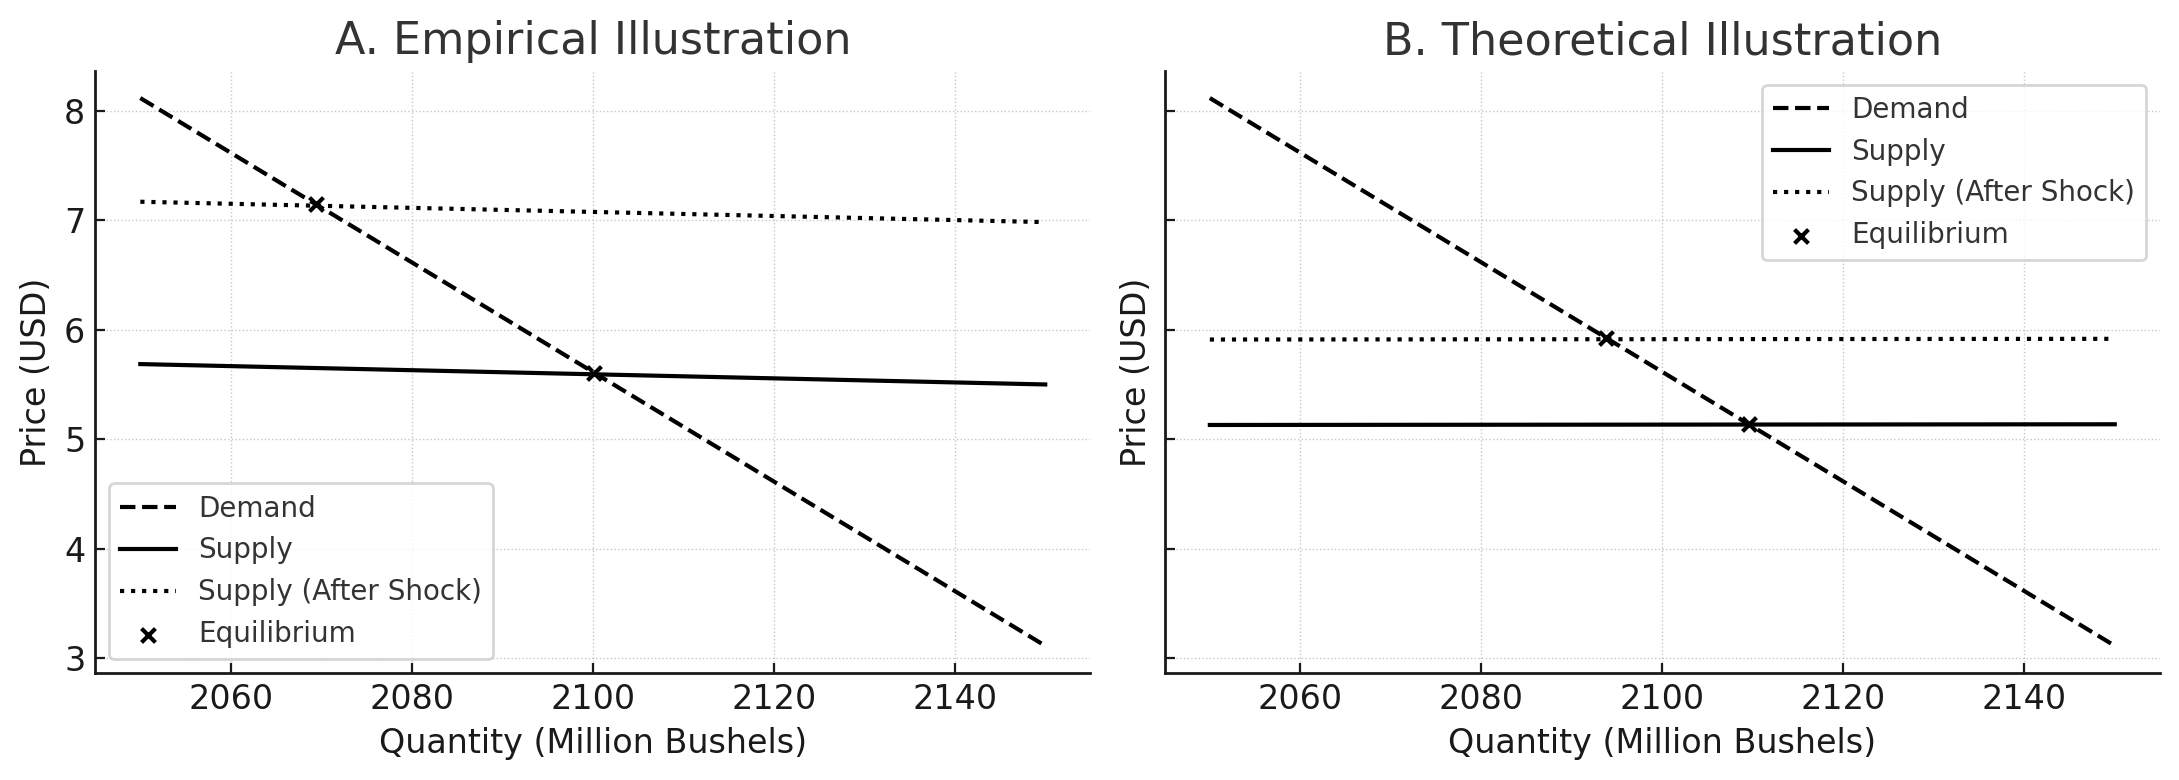
\includegraphics[width=0.9\linewidth]{Hakenes illustration.png}
\end{center}

\footnotesize
\begin{table}[h!]
\centering
\resizebox{0.8\linewidth}{!}{%
\begin{tabular}{lcc|cc}
\toprule
\textbf{Scenario} & \textbf{Qty (M bu)} & \textbf{CF (M kg CO\textsubscript{2}e)} & \textbf{Qty (M bu)} & \textbf{CF (M kg CO\textsubscript{2}e)} \\
\cmidrule(lr){2-3} \cmidrule(lr){4-5}
 & \multicolumn{2}{c}{\textbf{Empirical Model}} & \multicolumn{2}{c}{\textbf{Theoretical Model}} \\
\midrule
Before  & 2100.71 & 22859.68 & 2112.45 & 22983.46 \\
After   & 2068.38 & 22500.32 & 2096.36 & 22808.40 \\
$\Delta$ & ---     & \textbf{-359.36} & ---     & \textbf{-175.06} \\
\bottomrule
\end{tabular}}
\end{table}


\vspace{0.3em}
\scriptsize Source: Author's calculations based on USDA (2010--2017) and FAO data.


\vspace{0.5em}



\end{frame}
%---------------------------------------------

\begin{frame}{Results and Interpretation}
\footnotesize
\vspace{-2.0em}



\vspace{0.5em}
\textbf{Key Insights:}
\begin{itemize}
    \item Despite using the same demand curve, the empirical model estimates a larger emissions reduction (\(-359\) M kg CO\textsubscript{2}e) than the theoretical model (\(-175\) M kg CO\textsubscript{2}e).
    \item Discrepancy arises from supply modeling:  
        \begin{itemize}
            \item Empirical: OLS estimation on historical data; no explicit modeling of risk or equilibrium feedback.  
            \item Theoretical: derived from structural parameters, incorporating risk aversion, return volatility, and optimal capital allocation.
        \end{itemize}
    \item Theoretical framework embeds a consequentialist attribution, internalizing substitution effects and capital reallocation—muting output and emissions responses.
    \item Highlights the need to integrate behavioral and market feedbacks into footprint assessments for robust policy evaluation.
\end{itemize}

\end{frame}


%---------------------------------------------
\section{Responsibility \& Policy Implications}
\begin{frame}{Responsibility for Household Carbon Emissions}
\footnotesize
\vspace{-2.5em}
\textbf{Central Question:}  
How should household responsibility for climate change be defined, measured, and fairly attributed?\\
\vspace{0.5em}
\textbf{Attribution Logics:}
\begin{enumerate}
  \item \textbf{Control-based (GHG Protocol)}: 
    \begin{itemize}
      \footnotesize
      \item Emissions assigned to actors with operational control of sources (Scopes~1--2); producer-focused. 
      \item Upstream supply-chain emissions (Scope~3) typically excluded.
      \item Limited to operational control, often underestimates total responsibility.
      \item Under household lens: 10--20\% of national emissions assigned
      \item \textbf{Policy Implication:} 
        \begin{itemize}
          \item Focuses on direct emissions reduction; less effective for upstream supply chains.
          \item May incentivize offshoring emissions rather than reducing them.
        \end{itemize}
    \end{itemize}
  \end{enumerate}
  \end{frame}

\begin{frame}{Responsibility for Household Carbon Emissions (cont.)}
\footnotesize
\begin{enumerate}
  \setcounter{enumi}{1}
  \item \textbf{Consumption-based (LCA, EEIO)}: 
    \begin{itemize}
      \footnotesize

      \item \textbf{LCA:} Attributes responsibility to households by assigning them all direct and upstream emissions generated across a product’s entire life cycle, proportionally to their consumption of that product or service.
  \item \textbf{EEIO:} Links household final demand vector $\mathbf{F}$ to sectoral emissions via
    \[
      \mathbf{E} = \mathbf{C} (\mathbf{I} - \mathbf{A})^{-1} \mathbf{F}
    \]
      \item Under household lens: 60--80\% of national emissions assigned.
      \item \textbf{Policy Implication:} 
        \begin{itemize}
          \item Encourages individual climate responsibility through policies that use behavioral nudges to encourage sustainable consumption.
          \item Risks overstating household agency by ignoring structural and supply-side constraints.
        \end{itemize}
    \end{itemize}
    \end{enumerate}
    \end{frame}

\begin{frame}{Responsibility for Household Carbon Emissions (cont.)}
\footnotesize
\vspace{-3.0em}
\begin{enumerate}
  \setcounter{enumi}{2}
  \item \textbf{Consequentialist (Hakenes–Schliephake)}:
    \begin{itemize}
      \footnotesize
      \item Attributes household responsibility to the \textit{marginal causal impact} of its consumption and investment decisions on total emissions.
      \item Compares general equilibrium with the household present to the counterfactual without it, capturing direct and indirect market spillovers.
      \item Defines marginal impact footprint:
      \[
        fp_h = x \left( \phi q_h + (1-\phi)\frac{i_h}{c} \right)
      \]
      \item $\phi = \frac{b}{b + c^2 \alpha \sigma^2}$ allocates responsibility between consumption and investment.
      \item Higher $\alpha$ (risk aversion) or $\sigma^2$ (return variance) shifts responsibility toward consumption; greater substitutability amplifies investment effects.
      \item Can yield near-zero responsibility if actions are fully offset by others, avoiding over-attribution in static frameworks.
      \item \textbf{Policy Implication:}
        \begin{itemize}
          \item Aligns with structural mechanisms such as green financial regulation or carbon-intensity weighting of investment portfolios.
          \item Differentiates between symbolic and substantive household climate action.
        \end{itemize}
    \end{itemize}
\end{enumerate}
\end{frame}

\begin{frame}{Comparative Analysis of Attribution Principles}
\small
\vspace{-2.5em}
\begin{center}
  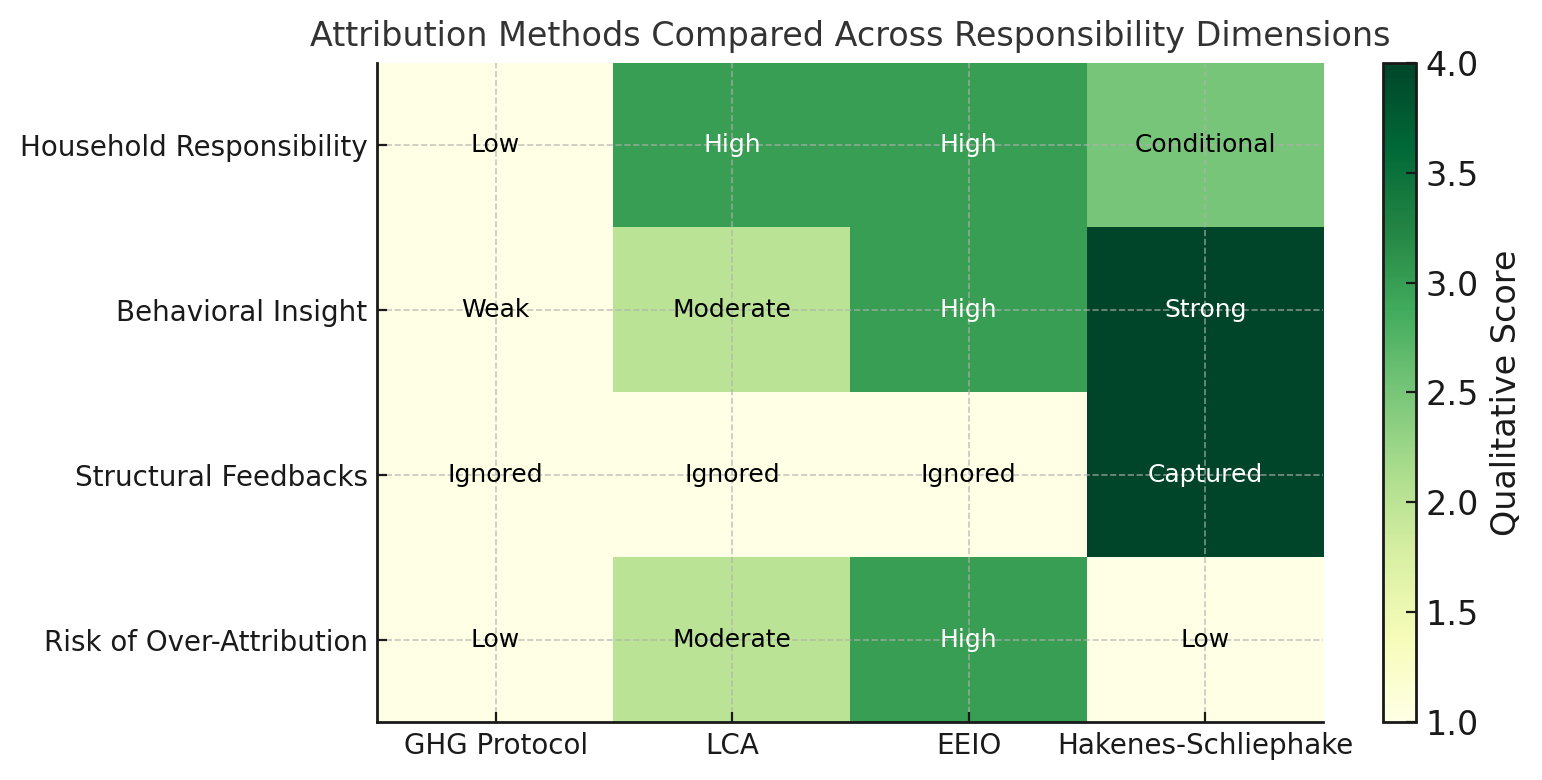
\includegraphics[width=0.75\linewidth]{Heatmap Res.png}

  \footnotesize
\textit{The heatmap compares attribution frameworks across behavioral relevance, structural sensitivity, and over-attribution risk.}
\end{center}
\footnotesize
\vspace{0.4em}
\textbf{Main finding:} Consequentialist attribution (H\&S) uniquely captures systemic feedbacks, avoiding double-counting while grounding responsibility in causal impact.
\end{frame}

\begin{frame}{Household Carbon Footprint Disparities}
  \vspace{-2.0em}
\centering
\begin{minipage}{0.45\linewidth}
    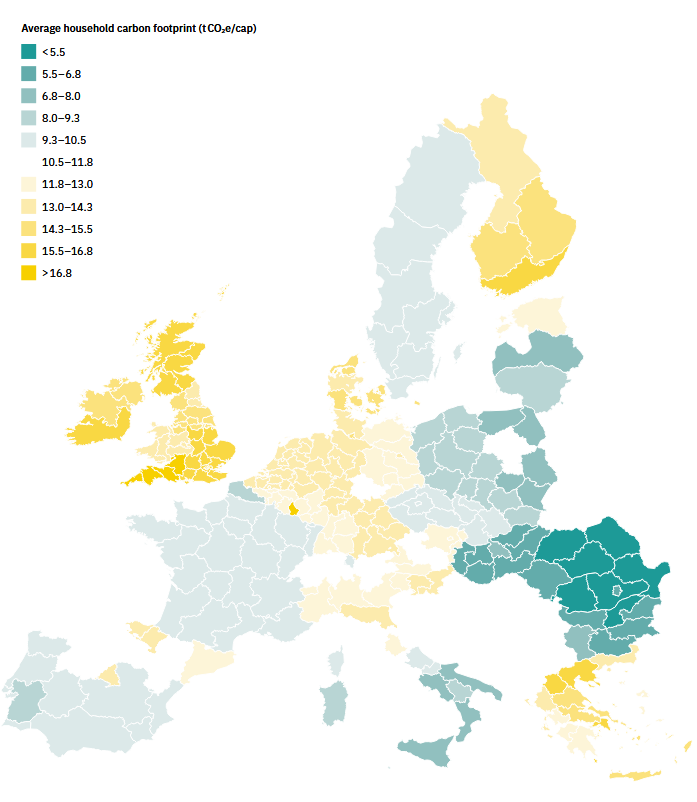
\includegraphics[width=\linewidth]{per capita world emissions.png}
\end{minipage}
\hfill
\begin{minipage}{0.45\linewidth}
    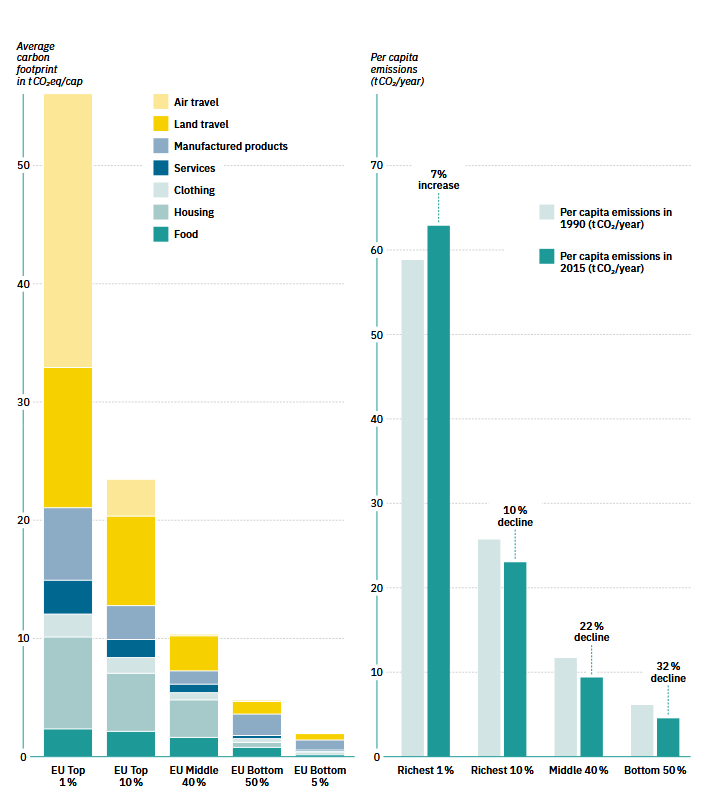
\includegraphics[width=\linewidth]{emission by income.png}
\end{minipage}

\vspace{0.5em}
\footnotesize
\textit{The heterogeneity in carbon footprints across regions and income groups determines the efficiency and equity outcomes of policy instruments.}
\end{frame}

%---------------------------------------------
\begin{frame}{Household Carbon Policy Instruments: Comparative Overview}
\footnotesize
\vspace{-2.5em}
%\textbf{Framing:} Policy efficacy hinges on the \textit{attribution framework}; methods determine not only the quantification of household emissions, but also the feasible policy levers and their distributive outcomes.

\vspace{0.8em}
\resizebox{\textwidth}{!}{%
\begin{tabular}{p{3.2cm} p{3.6cm} p{3.6cm} p{3.8cm}}
\toprule
\textbf{Instrument} & \textbf{Methodological Basis} & \textbf{Strengths} & \textbf{Limitations} \\
\midrule
Carbon Taxes & GHG Protocol (Scopes 1–2); extended by EEIO for consumption-based pricing & Price-based efficiency; scalable; fiscal integration & Regressive without redistribution; omits embedded emissions if Scope 3 excluded \\
\addlinespace
Product \& Appliance Standards & LCA with embedded carbon and durability criteria & Tech-driven efficiency gains; aligns with trade rules & Enforcement gaps; risk of excluding low-income users \\
\addlinespace
Investment-Based Tools & General equilibrium (Hakenes–Schliephake) with EEIO sectoral intensities & Targets capital-linked emissions; addresses top-income externalities & Data-intensive; politically sensitive in asset-heavy economies \\
\addlinespace
Behavioural Interventions & Behavioural economics; weakly embedded in static models & Low-cost, adaptive, socially contextual & Under-captured in conventional carbon metrics \\
\addlinespace
AI-Enabled Platforms & Hybrid EEIO–LCA with transaction-level data & Real-time tracking; personalised policy feedback & Digital divide; privacy and governance risks \\
\bottomrule
\end{tabular}
}
\end{frame}

%---------------------------------------------
\begin{frame}{Strategic Insights from Comparative Assessment}
\footnotesize
\textbf{Key Takeaways:}
\begin{itemize}
  \item Attribution logic is endogenous to policy design — \textit{what is measured constrains what can be mitigated}.
  \item Static, control-based approaches (GHG Protocol) facilitate fiscal and regulatory instruments but understate indirect and imported emissions.
  \item LCA and EEIO expand system boundaries, enabling product regulation and consumption-based taxation, but risk over-attribution absent behavioural or supply-side constraints.
  \item Equilibrium models capture inter-market spillovers and capital flows, offering distribution-sensitive interventions, particularly for high-wealth cohorts.
  \item Behavioural and AI tools bridge micro-level heterogeneity with adaptive policy targeting, but remain weakly institutionalised in formal carbon accounting.
\end{itemize}
\end{frame}

%---------------------------------------------
\begin{frame}{Conclusion: Method–Instrument Alignment}
\footnotesize
\textbf{Synthesis:}
\begin{itemize}
  \item No single instrument is universally optimal — efficiency, equity, and political feasibility trade-offs are shaped by the underlying attribution framework.
  \item Integration across methods is essential: \textit{fiscal} (tax), \textit{technological} (standards), \textit{financial} (investment), and \textit{behavioural} levers target distinct channels of household emissions.
  \item Economically coherent design requires aligning price signals, regulatory standards, and behavioural incentives within the structural constraints revealed by the chosen model.
\end{itemize}
\vspace{0.5em}
\textit{Implication for policy:} Incomplete or mismatched attribution undermines both cost-effectiveness and distributional legitimacy.
\end{frame}
%---------------------------------------------

\begin{frame}{Household Carbon Policy Instruments: Methods, Examples, and Economic Notes}
\scriptsize
\vspace{-3.0em}
\renewcommand{\arraystretch}{1.15}
\resizebox{\textwidth}{!}{%
\begin{tabular}{p{3.2cm} p{3.3cm} p{3.3cm} p{3.6cm}}
\toprule
\textbf{Instrument} & \textbf{Methodological Basis} & \textbf{Example Implementations} & \textbf{Features} \\
\midrule
\textbf{Carbon Taxes} & GHG Protocol (Scopes 1–2); EEIO for consumption-based pricing & Sweden: 130+ USD/tCO$_2$; Canada federal backstop; EU Border Carbon Adjustment & Internalises marginal social cost; scalable; regressive without revenue recycling; leakage risk if embedded emissions excluded \\
\addlinespace
\textbf{Product \& Appliance Standards} & Life Cycle Assessment (LCA); embedded carbon and durability metrics & EU Ecodesign Directive; Japan Top Runner; US Energy Star & Corrects efficiency market failures; harmonisable in trade policy; effectiveness depends on enforcement and affordability \\
\addlinespace
\textbf{Investment-Based Tools} & General Equilibrium (Hakenes–Schliephake) with EEIO sectoral intensities & EU ETS; California Carbon Allowance; ESG ETFs; Green Bonds & Targets capital allocation to low-carbon sectors; addresses emissions concentration; politically sensitive, data-intensive \\
\addlinespace
\textbf{Behavioural Interventions} & Behavioural economics; typically outside static carbon models & UK smart meter nudges; diet-shift campaigns; cookstove adoption programs & Low-cost demand adjustment; high social adaptability; persistence and measurement challenges \\
\addlinespace
\textbf{AI-Enabled Platforms} & Hybrid EEIO–LCA with transaction-level data integration & Moneythor tracker; Svalna app; Klima app & Real-time, marginal behaviour targeting; adaptive feedback; digital divide and privacy governance concerns \\
\bottomrule
\end{tabular}
}
\end{frame}


\begin{frame}{Synthesis: Economic Logic and Strategic Trade-Offs}
\footnotesize
\begin{itemize}
  \item \textbf{Attribution methods determine instrument choice:}  
    \begin{itemize}
      \item GHG Protocol $\rightarrow$ direct price signals (carbon taxes, fuel levies).
      \item LCA $\rightarrow$ product-level regulation (standards, eco-design).
      \item EEIO $\rightarrow$ consumption-based taxes, trade adjustments.
      \item General equilibrium $\rightarrow$ capital market instruments.
      \item Behavioural/AI $\rightarrow$ adaptive, personalised demand-side measures.
    \end{itemize}
  \item \textbf{Core trade-offs:}  
    Taxes = allocatively efficient but potentially regressive.  
    Standards = technology-forcing, risk of exclusion.  
    Investment tools = target high-emission wealth segments, politically sensitive.  
    Behavioural = socially embedded, hard to monetise.  
    AI = granular and dynamic, constrained by digital equity.
  \item \textbf{Strategic implication:}  
    No single instrument optimises efficiency, equity, and political feasibility.  
    An optimal portfolio integrates complementary tools, each grounded in the correct attribution logic, to maximise mitigation while maintaining fairness and public acceptance.
\end{itemize}
\end{frame}


\begin{frame}{Conclusion}
\footnotesize
\textbf{Key Takeaways:}
\begin{itemize}
    \item Household carbon footprints are highly sensitive to \textbf{attribution framework}:
    \begin{itemize}
        \item GHG Protocol, LCA $\rightarrow$ lower footprints, focus on direct use.
        \item EEIO, general equilibrium $\rightarrow$ higher footprints via supply chains, market spillovers, capital allocation.
    \end{itemize}
    \item Method choice \textbf{determines policy alignment}:
    \begin{itemize}
        \item GHG Protocol $\rightarrow$ direct fuel/energy pricing.
        \item LCA $\rightarrow$ product and appliance standards.
        \item EEIO $\rightarrow$ upstream interventions, border carbon adjustments.
        \item GE model $\rightarrow$ investment-based and capital-sensitive instruments.
    \end{itemize}
    \item Ensuring \textbf{internal consistency} between accounting method, policy instrument, and financing strategy is critical for efficiency and fairness.
\end{itemize}

\vspace{0.4em}
\textbf{Future Work:}
\begin{itemize}
    \item Integrate micro-level household data, dynamic GE extensions, and behavioural/digital mechanisms.
\end{itemize}

\vspace{0.4em}
\textbf{Final Note:}  
Methodological choices are not neutral—they shape the scale, focus, and equity of household decarbonisation policy.
\end{frame}

\end{document}


